\subsection{Inductances}
\label{sec:inductances}

The step-by-step method of inductance extraction is found in Section \ref{sec:extraction}. This section deals with the reasoning behind investigating particular traces.

\begin{figure}[H]
	\centering
	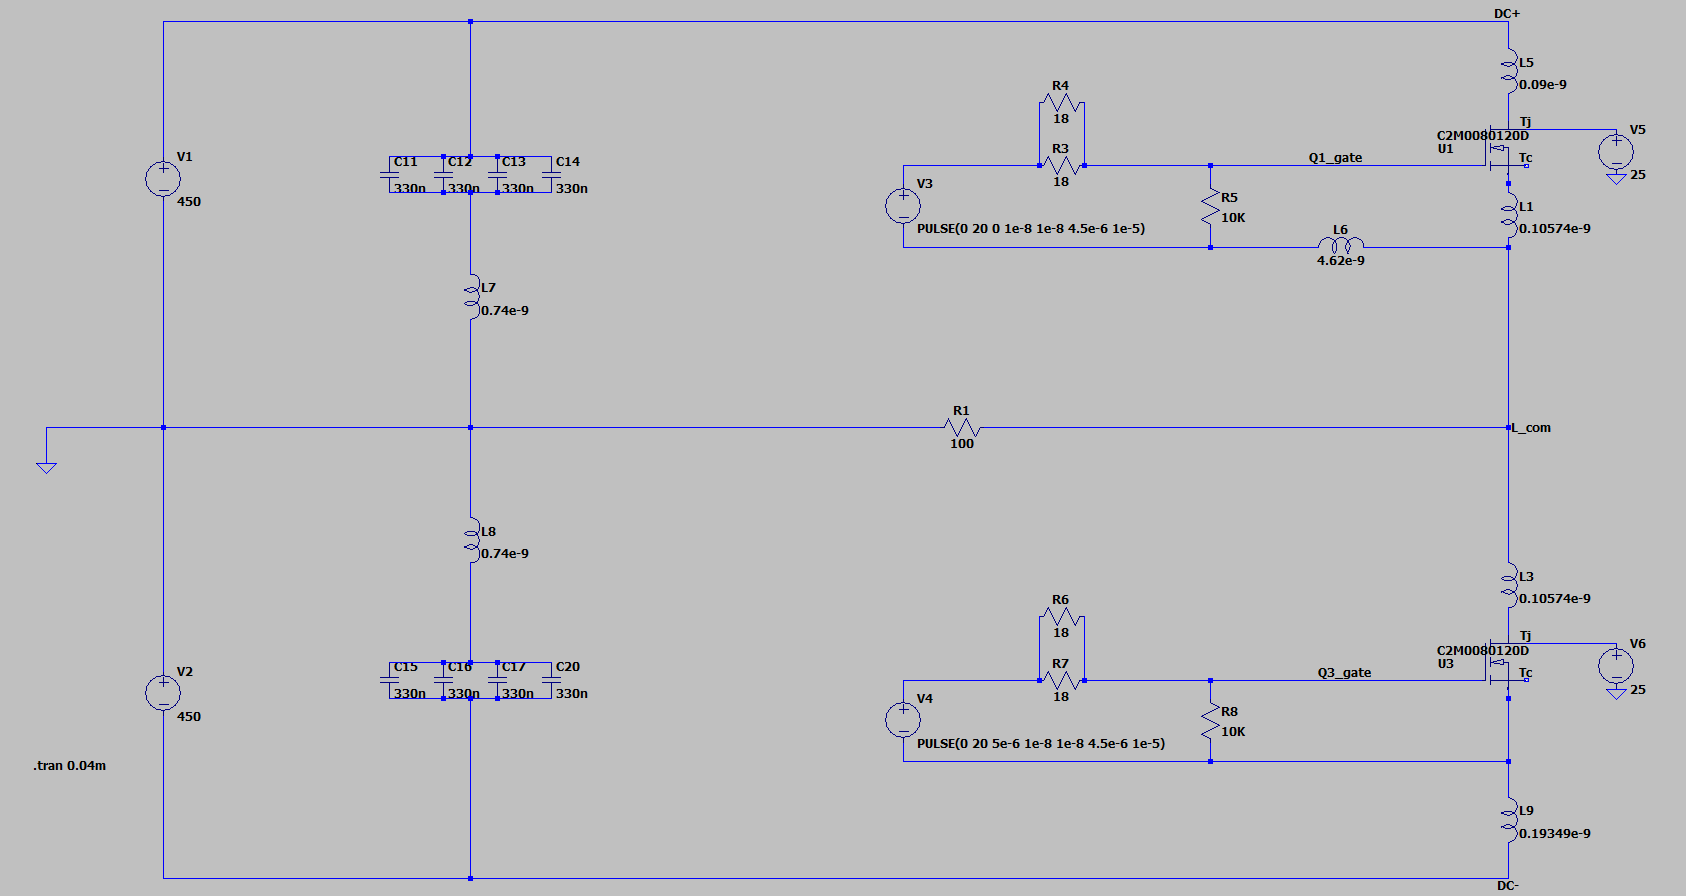
\includegraphics[width=\textwidth]{pictures/implementation/ind/spice_ind_1.PNG}
	\caption{Spice model with inductances}
	\label{fig:spice_ind}
\end{figure}

\subsubsection{Q1 drain}
\label{sec:Q1_drain}

The track between the drain terminal of Q1 and the capacitor bank C11-C12-C13-C14 is a part of interest. It is not only the DC+ power rail but Section \ref{sec:oscillators} details why the drain inductance is so critical. Section \ref{sec:extraction} details the position of the terminals in the layout. It is apparent that Q1 drain and the top of the capacitor bank is very close to each other on the layout and it manifests in a stray inductance value of $0.09 nH$ and negligible resistance.

\subsubsection{Q1 and Q3 gate}
\label{sec:q1_q3_gate}

Q1 and Q3 gate is driven via resistors very closely placed to the terminals. Their inductances proved to be extremely low, in the $pF$ order, therefore they were left out of the model. Figure \ref{fig:q1_gate} highlights the aforementioned distance at Q1. Q3 is symmetrical on the bottom side of the board.

\begin{figure}[H]
	\centering
	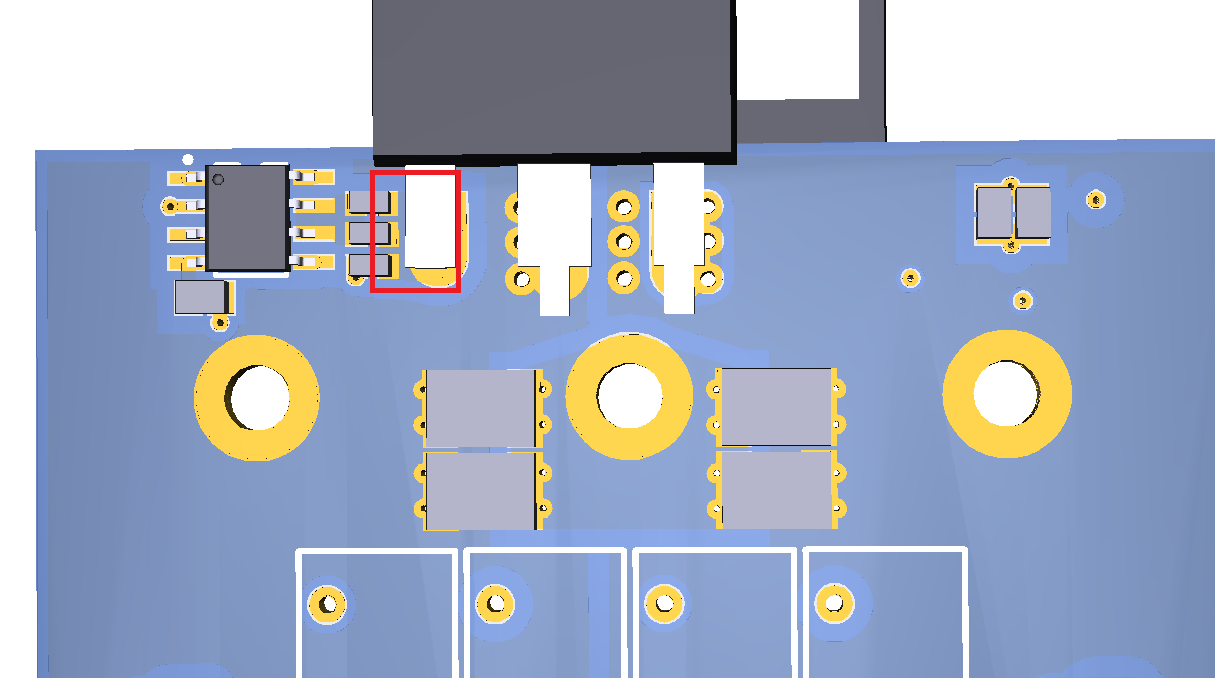
\includegraphics[width=\textwidth]{pictures/implementation/ind/Q1_gate.png}
	\caption{Distance between gate pin and drive line resistors}
	\label{fig:q1_gate}
\end{figure}

\subsubsection{Q1 source and Q3 drain}

The point L\_com in Figure \ref{fig:spice_ind} is a virtual point. It was inserted to connect the load nonexistent in the layout. It splits the L net in two, so for the sake of maintaining symmetry, the extracted inductance was also split in two. This yields a value of $0.106 nH$ for each of them with a practically negligible resistance of $0.00004 \ohm$.

\subsubsection{Q1 source and R5 lower pad}
\label{sec:q1_r5}

The gate signal return path is demonstrated in Figure \ref{fig:q1_r5}. The left small mark is the via to the bottom pad of R5. The total inductance extracted is $4.73 nH$. Since L1 is already represented in that loop, L6 got the value of $4.73 - 0.106 = 4.62 nH$. This may not matter much as L1 is about 2\% of the loop inductance but demonstrates the principle of partitioning a circuit.

\begin{figure}[H]
	\centering
	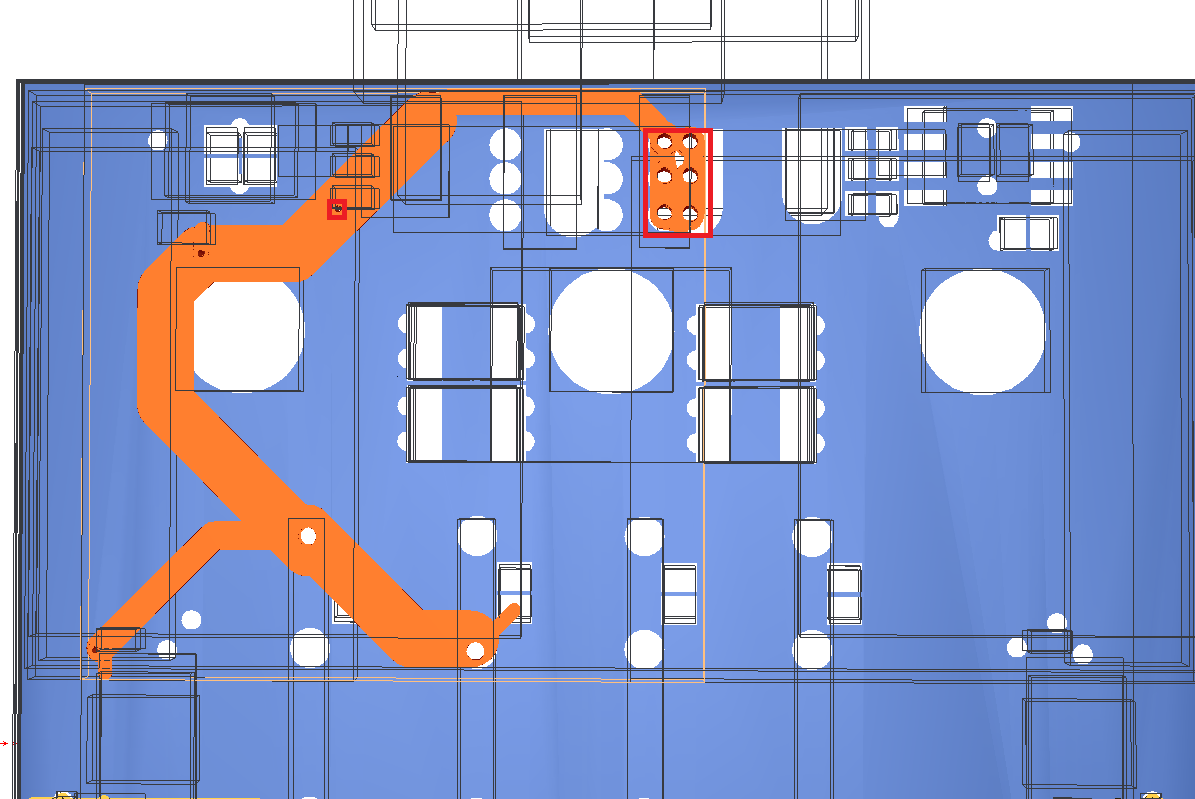
\includegraphics[width=\textwidth]{pictures/implementation/ind/q1_r5.png}
	\caption{Q1 gate signal return path}
	\label{fig:q1_r5}
\end{figure}

\subsubsection{Q3 source and DC-}
\label{sec:q3_source}

Inductance between the source of Q3 and the DC-rail is about as large as between $Q1_{source}$ and $Q3_{drain}$, $0.193 nH$.

\subsubsection{Capacitor banks}
\label{sec:cap_banks}

The inductance was split in two to accommodate the ground point of the symmetrical voltage sources. This yields $L7 = L8  = 0.74 nH$, with a resistance of $0.0013 \ohm$ for each.

\subsubsection{Waveforms}
\label{sec:ind_waveforms}

The simulated waveforms look plausible. Some cross-coupling can be seen at the moment of the switching but this is not enough to trigger false turn on-off cycles.

Figure \ref{fig:ind_gates_1} shows two whole cycles as an overview, Figure \ref{fig:ind_gates_2} shows the transient where $ Q1\ V_{GS}$ turns off, Figure \ref{fig:ind_gates_3} depicts the other end of that cycle. Figure \ref{fig:ind_load} demonstrates the voltage and current of the load.

\begin{figure}[H]
	\centering
	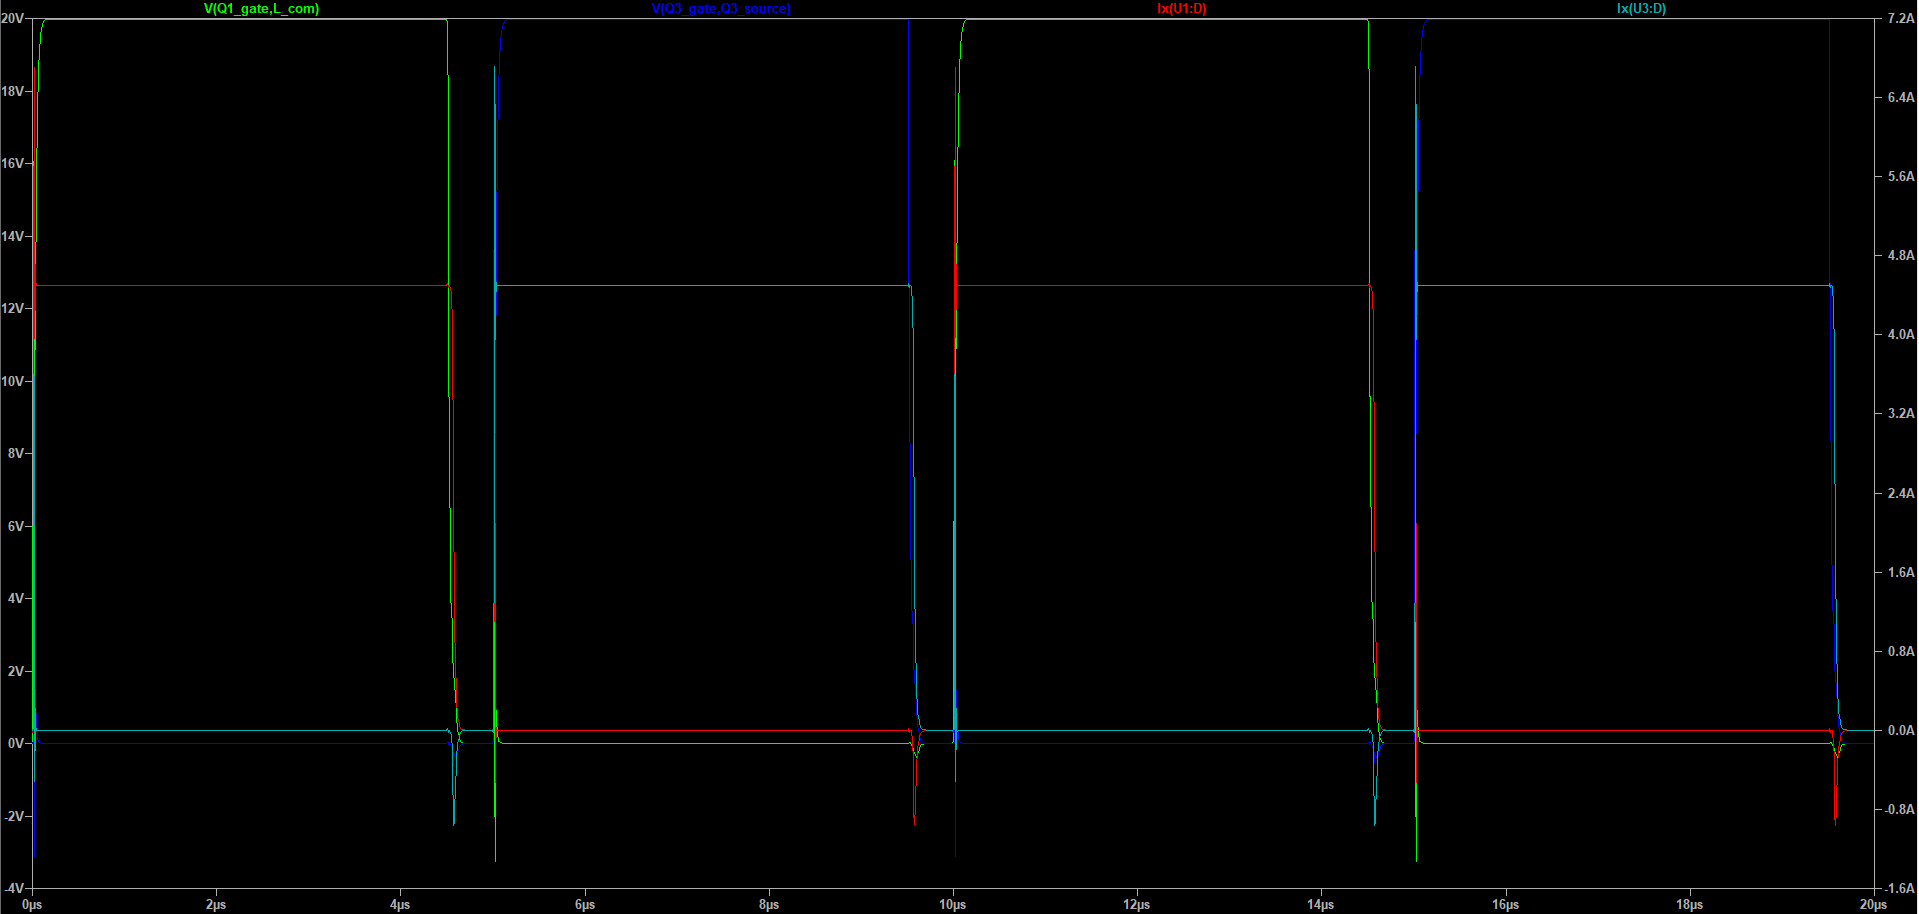
\includegraphics[width=\textwidth]{pictures/implementation/ind/ind_gates_1.PNG}
	\caption{Overview of the gate voltages and drain currents}
	\label{fig:ind_gates_1}
\end{figure}

\begin{figure}[H]
	\centering
	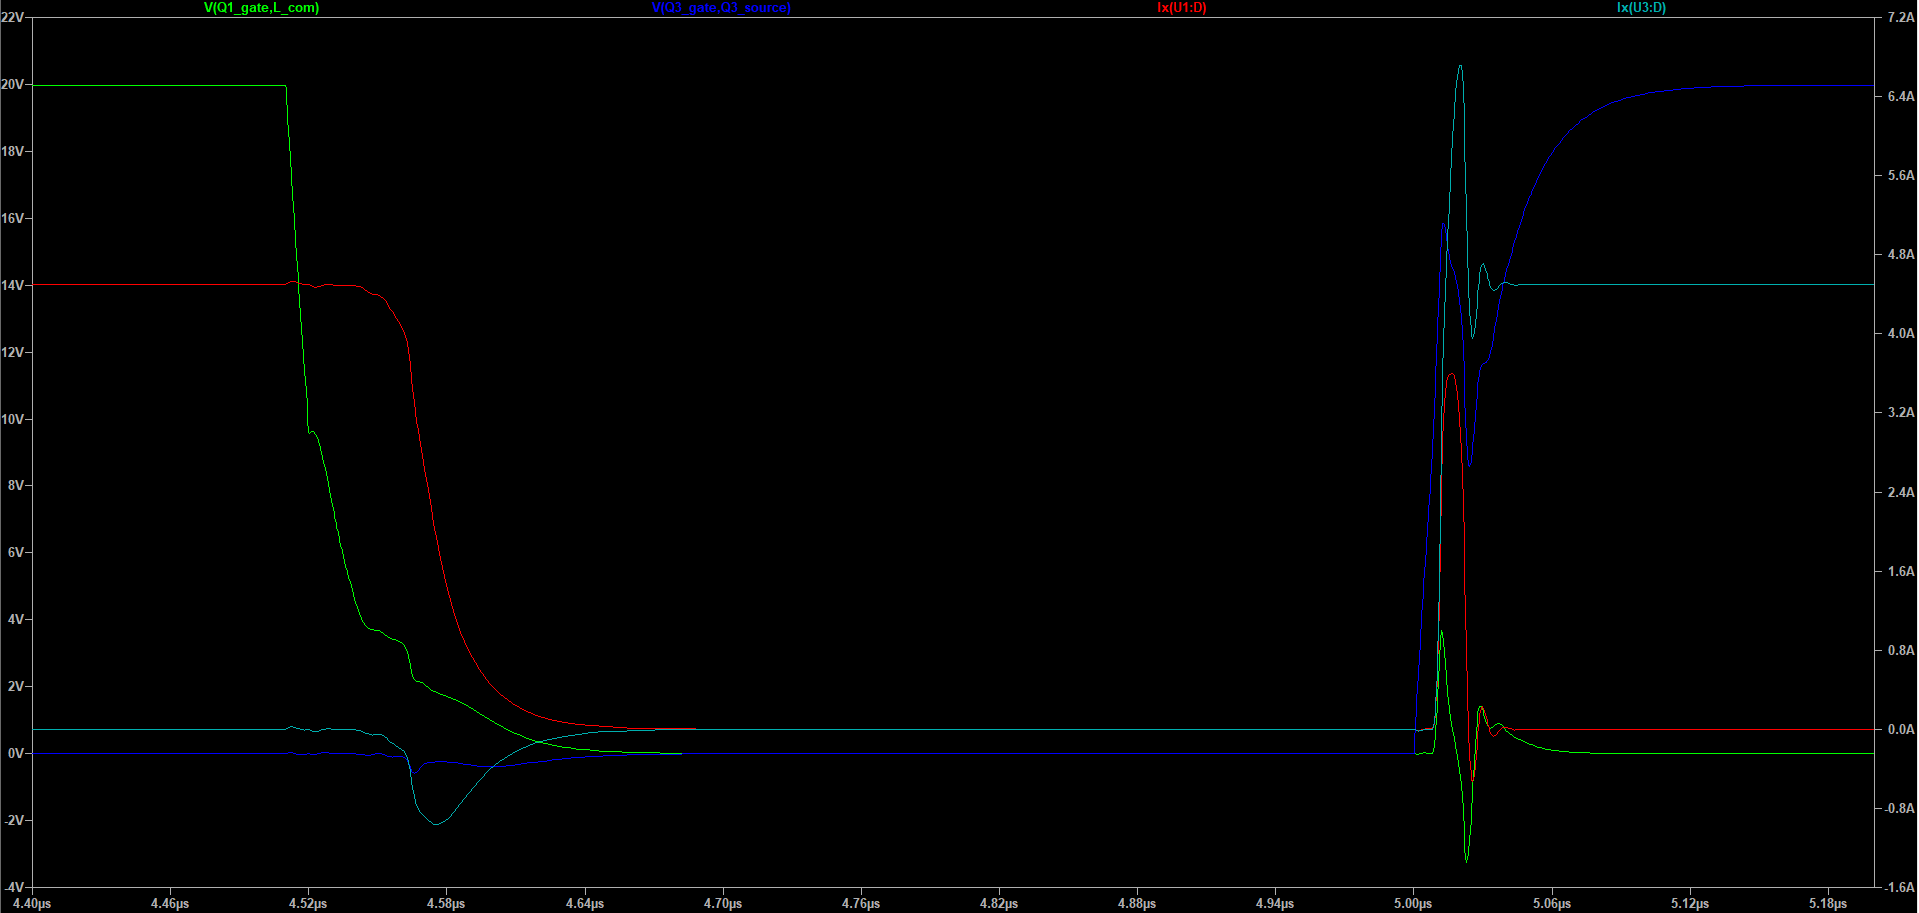
\includegraphics[width=\textwidth]{pictures/implementation/ind/ind_gates_2.PNG}
	\caption{Q1 turn off transient, gate voltages and drain currents}
	\label{fig:ind_gates_2}
\end{figure}

\begin{figure}[H]
	\centering
	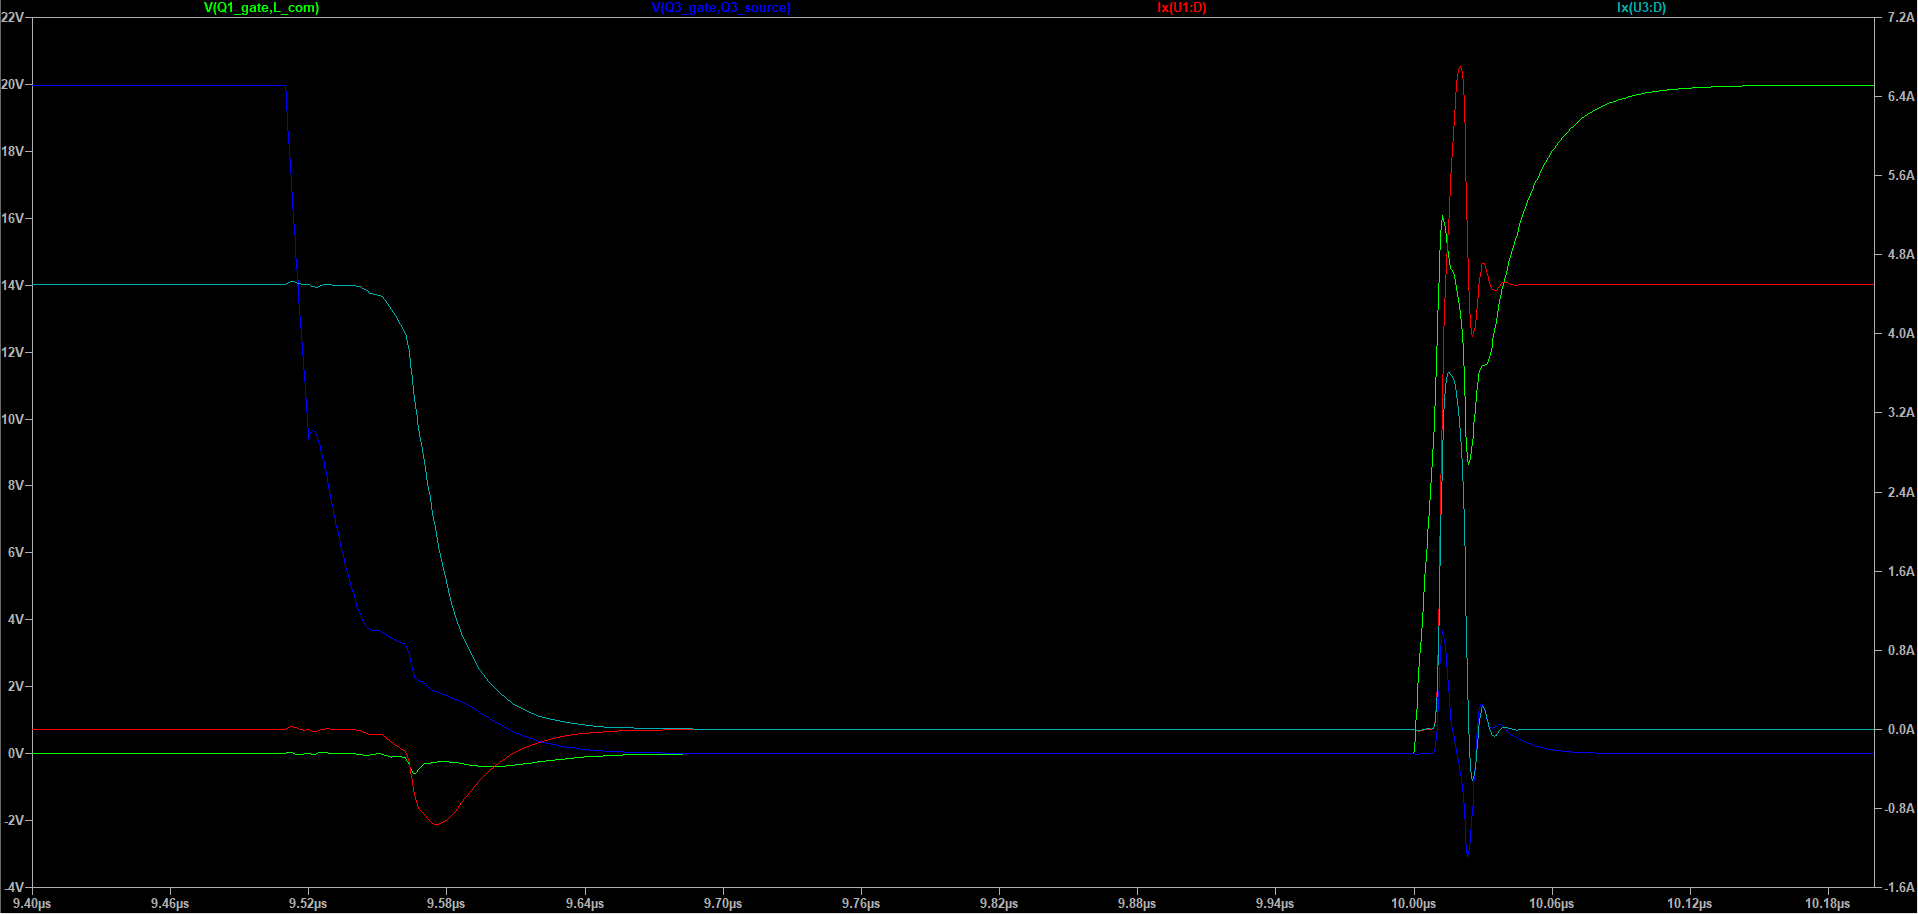
\includegraphics[width=\textwidth]{pictures/implementation/ind/ind_gates_3.PNG}
	\caption{Q3 turn off transient, gate voltages and drain currents}
	\label{fig:ind_gates_3}
\end{figure}

\begin{figure}[H]
	\centering
	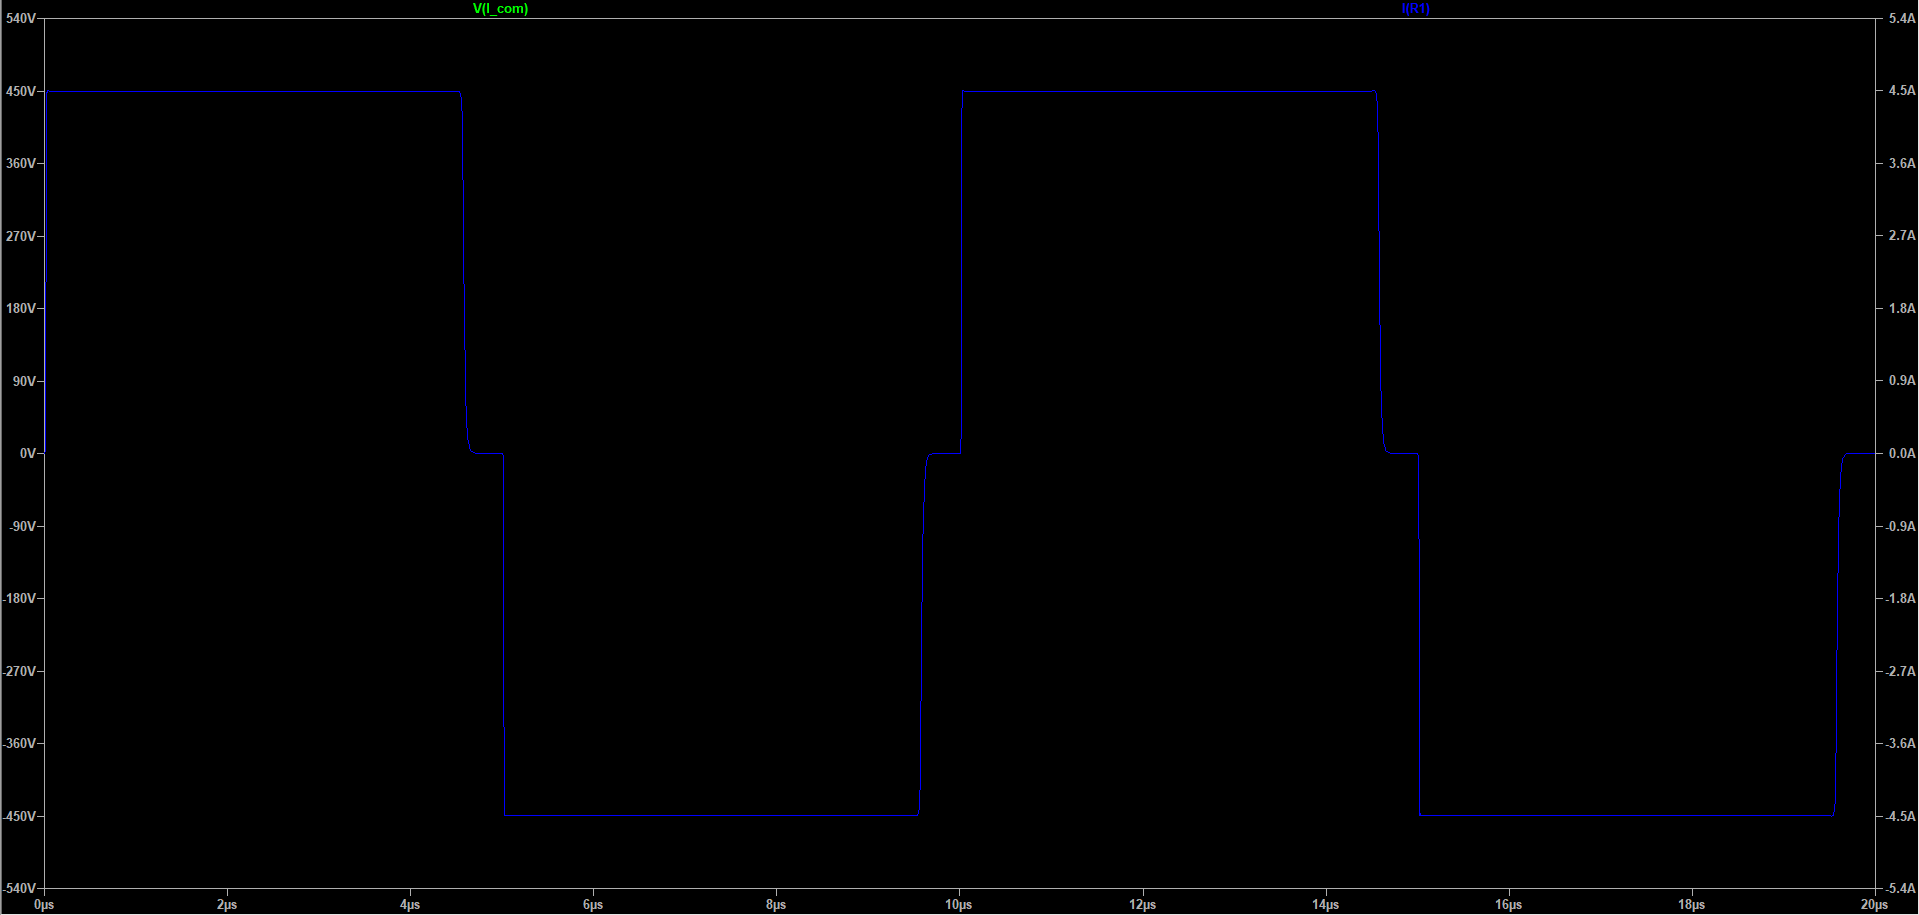
\includegraphics[width=\textwidth]{pictures/implementation/ind/ind_load.PNG}
	\caption{Voltage and current waveforms of the resistor overlap}
	\label{fig:ind_load}
\end{figure}